\documentclass{article}
\usepackage[papersize={6.95in,4.75in},margin=9pt]{geometry}
% Shared visual grammar for FIGURE_FREEZE_V1.
% One blue family + grayscale. Meaning also encoded by shape/border.
\usepackage[T1]{fontenc}
\usepackage{lmodern}
\usepackage{amsmath,amssymb}
\usepackage{tikz}
\usetikzlibrary{arrows.meta,positioning,fit,calc,matrix}

\definecolor{ink}{HTML}{22272B}
\definecolor{muted}{HTML}{5C6770}
\definecolor{rule}{HTML}{B7C0C7}
\definecolor{band}{HTML}{F3F5F7}
\definecolor{accent}{HTML}{2E5A88}
\definecolor{accentfill}{HTML}{E7F0F6}

\tikzset{
  arr/.style={-{Latex[length=2.1mm,width=1.6mm]}, line width=0.6pt, draw=ink},
  arrd/.style={-{Latex[length=2.1mm,width=1.6mm]}, densely dashed, line width=0.6pt, draw=muted},
  figbase/.style={
    font=\small\selectfont,
    color=ink,
    line cap=round,
    line join=round,
  },
  box/.style={
    draw=ink, line width=0.55pt,
    rounded corners=1.4pt,
    inner sep=3.6pt,
    align=center,
    text=ink,
  },
  boxplain/.style={box, fill=white},
  boxband/.style={box, fill=band, draw=rule},
  boxaccent/.style={box, fill=accentfill, draw=accent, line width=0.7pt},
  untrusted/.style={box, densely dashed, draw=muted, fill=white},
  badge/.style={
    font=\footnotesize\selectfont,
    inner sep=2.2pt,
    align=center,
    draw, line width=0.6pt,
    rounded corners=1.1pt,
  },
  badgeexact/.style={badge, fill=accentfill, draw=accent},
  badgesubst/.style={badge, fill=white, draw=accent, densely dashed},
  badgerule/.style={badge, fill=white, draw=ink, double, double distance=1.05pt},
  badgeunk/.style={badge, fill=white, draw=muted, dotted},
  badgerefuse/.style={badge, fill=white, draw=ink, dashed},
  lab/.style={font=\footnotesize\selectfont, text=muted, align=center, inner sep=1pt},
  head/.style={font=\normalsize\bfseries\selectfont, text=accent, align=center},
  axislab/.style={font=\footnotesize\selectfont, text=ink},
}

\pagestyle{empty}
\setlength{\parindent}{0pt}
\begin{document}
\centering
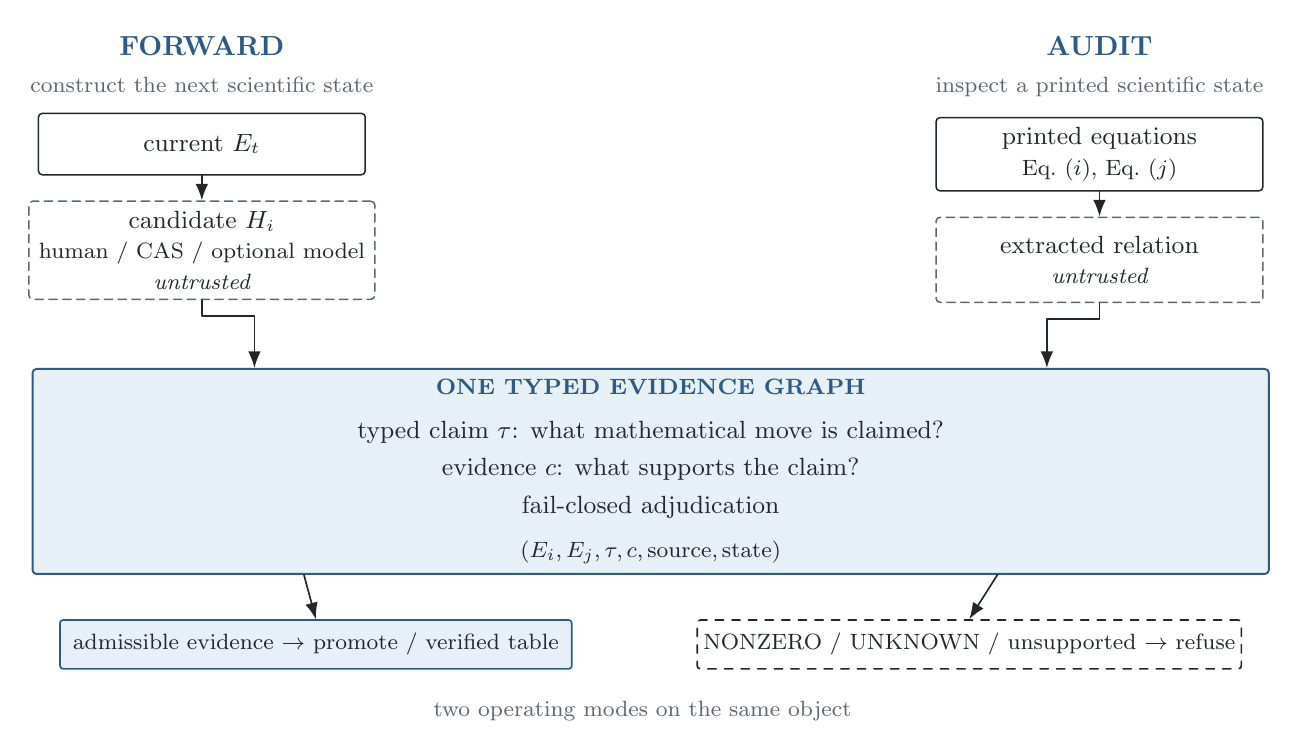
\begin{tikzpicture}[figbase]
  \node[head] (hf) at (2.15,0) {FORWARD};
  \node[lab, below=3pt of hf] (hfs) {construct the next scientific state};
  \node[boxplain, below=6pt of hfs, minimum width=4.15cm, minimum height=0.78cm] (et)
    {current $E_t$};
  \node[untrusted, below=9pt of et, minimum width=4.15cm, minimum height=1.08cm] (hi)
    {candidate $H_i$\\{\footnotesize human / CAS / optional model}\\{\footnotesize\itshape untrusted}};

  \node[head] (ha) at (13.55,0) {AUDIT};
  \node[lab, below=3pt of ha] (has) {inspect a printed scientific state};
  \node[boxplain, below=6pt of has, minimum width=4.15cm, minimum height=0.78cm] (eq)
    {printed equations\\{\footnotesize Eq.~$(i)$, Eq.~$(j)$}};
  \node[untrusted, below=9pt of eq, minimum width=4.15cm, minimum height=1.08cm] (rel)
    {extracted relation\\{\footnotesize\itshape untrusted}};

  \draw[arr] (et) -- (hi);
  \draw[arr] (eq) -- (rel);

  \path (hi.south) -- (rel.south) coordinate[midway] (mid);
  \node[boxaccent, below=24pt of mid, minimum width=15.7cm, minimum height=1.92cm, align=center] (core) {%
    {\footnotesize\bfseries\color{accent}ONE TYPED EVIDENCE GRAPH}\\[5pt]
    typed claim $\tau$: what mathematical move is claimed?\\[2.5pt]
    evidence $c$: what supports the claim?\\[2.5pt]
    fail-closed adjudication\\[5pt]
    {\footnotesize $(E_i,E_j,\tau,c,\text{source},\text{state})$}};

  \draw[arr] (hi.south) -- ++(0,-0.20) -| ($(core.north west)!0.18!(core.north east)$);
  \draw[arr] (rel.south) -- ++(0,-0.20) -| ($(core.north west)!0.82!(core.north east)$);

  \node[badgeexact, below=16pt of core.south west, anchor=north west, xshift=0.35cm,
        minimum width=6.5cm, minimum height=0.62cm] (ok)
    {admissible evidence $\rightarrow$ promote / verified table};
  \node[badgerefuse, below=16pt of core.south east, anchor=north east, xshift=-0.35cm,
        minimum width=6.5cm, minimum height=0.62cm] (no)
    {NONZERO / UNKNOWN / unsupported $\rightarrow$ refuse};

  \draw[arr] ($(core.south west)!0.22!(core.south east)$) -- (ok.north);
  \draw[arr] ($(core.south west)!0.78!(core.south east)$) -- (no.north);

  \node[lab, below=10pt of $(ok.south)!0.5!(no.south)$] {two operating modes on the same object};
\end{tikzpicture}
\end{document}
